% \KZ{It's better to break up this long file into sections. I think the word ``memory'' should appear in the paper title.}
\section{Introduction}

Mental health issues represent a significant challenge in contemporary society. According to the World Health Organization (WHO)~\cite{Freeman2022TheWM}, approximately 298 million individuals are affected by depressive disorders, which are the most prevalent issue of mental disorders among adults. Concurrently, many mental health systems are characterized by substantial deficiencies and imbalances in resources and services~\cite{Freeman2022TheWM}. This situation highlights the urgent need for more effective automated methods for the detection and diagnosis of depression, which would lead to better allocation of medical resources.

Among various automated diagnostic approaches, conversational agents (CAs) have emerged as particularly effective due to their cost efficiency, time-saving capabilities, and ability to maintain user anonymity~\cite{Ma2023UnderstandingTB}. CAs are especially valuable in the diagnosis of mental illnesses, where the process is more complex than diagnosing physical conditions, which can often be confirmed through test reports. Mental health diagnoses rely heavily on qualitative information obtained through patient interactions, which presents unique challenges compared to the more straightforward use of structured electronic medical records (EMRs)~\cite{Li2024AgentHA}. Additionally, in contrast to self-assessment chatbots~\cite{Jaiswal2019VirtualHQ}, conversational agents powered by large language models (LLMs)~\cite{chen2023llmempoweredchatbotspsychiatristpatient} demonstrate a greater propensity to offer emotional support and apply advanced professional skills to enhance the accuracy and effectiveness of diagnostic tasks.
\begin{figure}[!t]
    \centering
    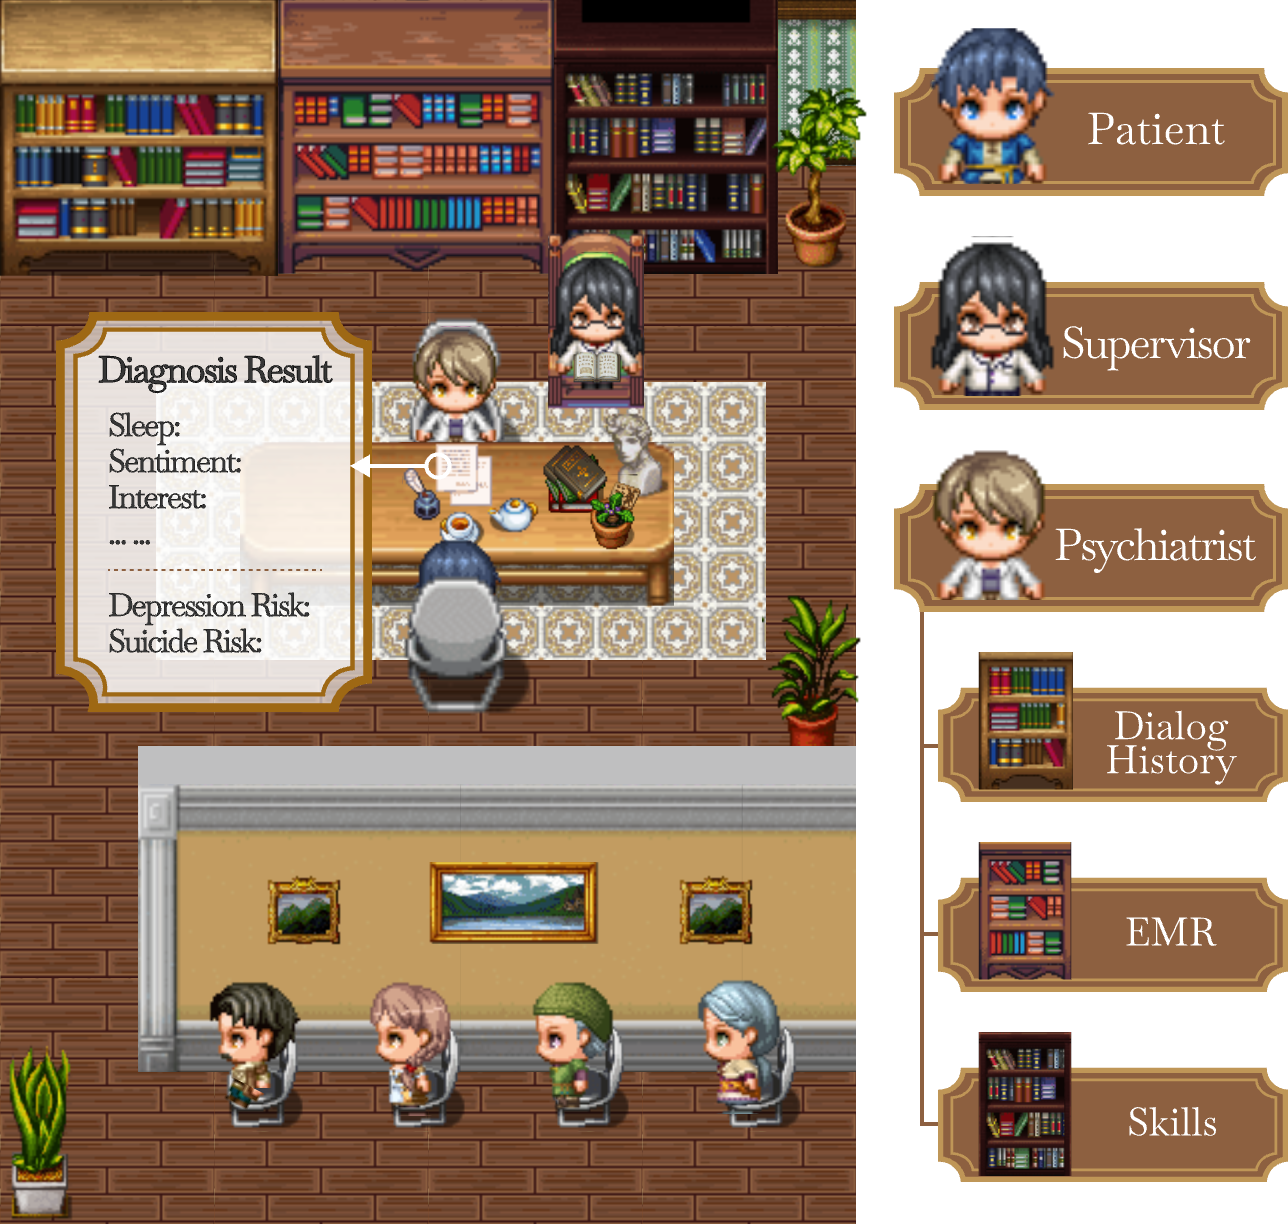
\includegraphics[width=1\linewidth]{fig/demo.png}
    \caption{\textbf{Agent Mental Clinic (\system).} The symptom list is collected during the conversation between the psychiatrist agent and the patient agent, with the guidance of the supervisor. Dialog History, Electronic Medical Records (EMR), and Skills are hierarchical memory layers of the psychiatrist agent. These layers are progressively refined throughout the depression diagnosis session.}
    \label{fig:demo}
\end{figure}



\begin{figure*}[!t]
    \centering
    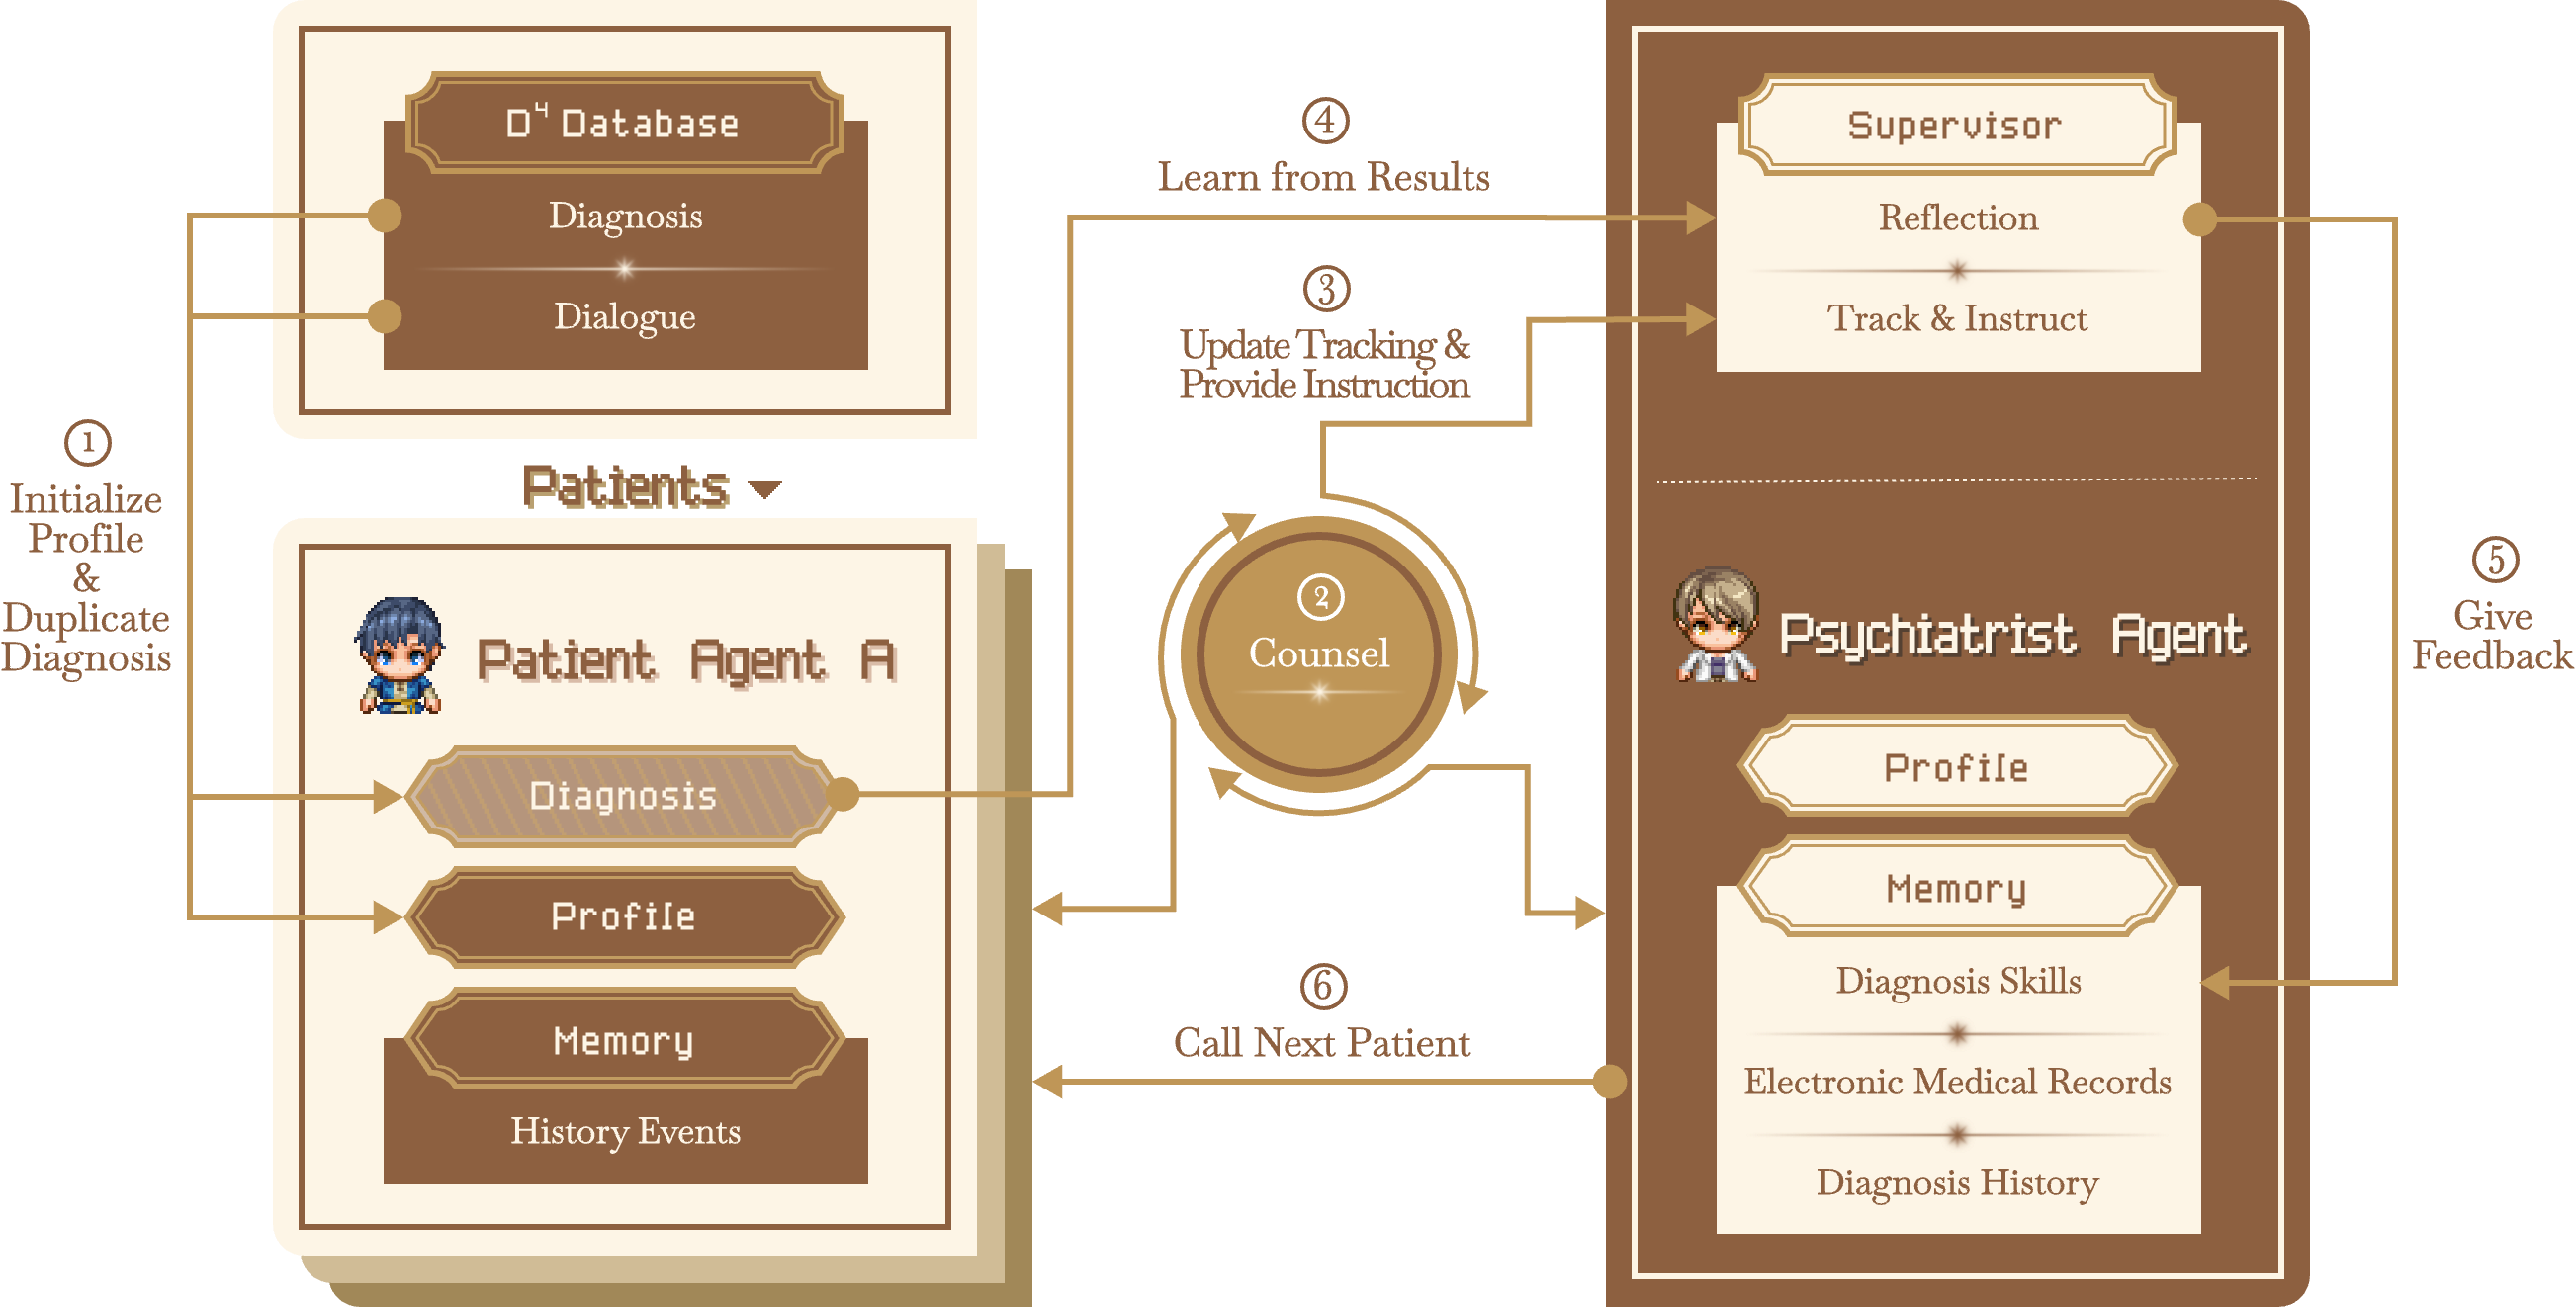
\includegraphics[width=1\linewidth]{fig/system_v8.png}
    \caption{\textbf{The overview of \system.} Agents are divided into patient agents and psychiatrist agents, while the supervisor plugin is attached to the psychiatrist agents to control the dialogue process. D4 database is a dataset including patient portraits, doctor-patient dialogue, and patients' diagnostic summaries. %\KZ{I thought we agreed to take the D4 database out of the patient box? And rename supervisor plugin to ``dialogue state control unit''? Don't say Patient Agent A, instead say Patient \#1, with a line of small words ``Patients'' on top of the whole stack of patients.}
    }
    \label{fig:overview}
\end{figure*}


Despite the strong performance of LLM-empowered conversational agents (CAs) in various conversation-based tasks~\cite{wu2023autogenenablingnextgenllm, Shi2023LLMMiniCEXAE, chen2023llmempoweredchatbotspsychiatristpatient}, the inherent biases within LLMs~\cite{yeh-etal-2023-evaluating, xu2024prideprejudicellmamplifies} remain challenging, even with the use of advanced prompting techniques. To be specific, in the mental health domain, previous research has revealed that 1) LLMs exhibit a preference for certain strategies~\cite{kang2024largelanguagemodelsgood, chen2023llmempoweredchatbotspsychiatristpatient}, such as emotion and sleep-related symptoms. 2) In diagnosis sessions, LLMs prefer to ask all the questions in one turn rather than step by step, and come to a diagnosis conclusion in several turns.~\cite{chen2023llmempoweredchatbotspsychiatristpatient} 3) LLMs might overlook the potential mental states of patients~\cite{jin2024psyevalsuitementalhealth}. The bias of LLMs harms their effectiveness in tasks like providing emotional support and conducting diagnosis conversations.  
%\MY{Can you cite siyuan's paper and say a standard depression diagnosis dialogue should be 1)the capability to interrogate all core depression symptoms in a conversation (symptoms checklist); 2)to ascertain the severity of specific symptoms (disease severity). However, current LLMs still fall in short xxxx}\

These limitation of LLMs emphasizes the necessity of dynamic prompt modification and the development of novel generative agents~\cite{Park2023GenerativeAgents}. These agents can maintain long-term coherence in simulating human behavior by managing expansive memories. The design of memory structures~\cite{zhang2024surveymemorymechanismlarge} allows these agents to sustain coherence and stimulate their self-evolution~\cite{zhang2024training, zhang2024surveymemorymechanismlarge}, demonstrating effectiveness in reducing LLM biases and enhancing performance across various complex conversational tasks~\cite{qian2024chatdevcommunicativeagentssoftware,wu2023autogenenablingnextgenllm, Li2024AgentHA}.






Although the effectiveness of memory structure in agent dialogue simulation is widely acknowledged, most approaches of memory retrieval still rely on previous criteria~\cite{Park2023GenerativeAgents}, including relevance, recency, and importance, which proves inadequate in mental health diagnosis conversation since 1) GPT-generated importance scores often fail to align with the requirements of realistic depression diagnostic process. 2) Recency scores are not effective without time simulation in diagnosis simulation. 3) The prevalent Top-$k$ retrieval method is insufficient in increasing the diversity of memories accessed by agents, leading to redundancy as experiments progress. The redundancy not only increases the time-consuming of retrieval operations but also limits the potential for optimization.


To further explore the effectiveness of memory modules in agent dialogue simulation, we propose a novel conversational agents simulation system \textbf{A}gent \textbf{M}ental \textbf{C}linic (\system), focusing on depression diagnosis conversation sessions (\figref{fig:overview}). To replicate the diagnosis procedure in real life, we utilized D$^4$ dataset~\cite{yao-etal-2022-d4}, a Chinese depression diagnosis dialogue dataset based on user portraits collected in real-world settings to evaluate the depression diagnosis accuracy of the psychiatrist agents. The experimental results indicate that the psychiatrist agents can enhance their performance after reflecting and learning from training cases, and achieve a higher diagnosis accuracy on unknown cases.
The key contribution of this paper is as follows:

\begin{itemize}
    \item We introduce a novel conversational agent simulation system to imitate the diagnostic sessions between patient agents and psychiatrist agents, This system generates realistic depression diagnostic conversations between agents, providing a promising method for training intern psychiatrists and for conducting preliminary depression risk screening on individuals exhibiting depressive symptoms.
    \item We propose an innovative memory structure and a retrieval module to enhance the utilization of skills generated by the agents. This improvement suggests a direction for future optimization in both depression diagnosis and the simulation of diagnostic conversations.
    \item Experiment results based on depression diagnosis conversation collected from real-life scenarios demonstrate the effectiveness of our \system~system, with an average improvement of 6.05 percent in depression diagnosis, and 1.8 percent in suicide prediction. Our framework can be applied in other specific domains with only a limited number of finely labeled cases available for training.
    %\MY{list a few numbers here and on what metrics}
    %\KZ{How effective?}\MY{can we compare both dialogue quality and diagnosis accuracy} 
    
\end{itemize}
